\documentclass[conc-doc]{subfiles}

\begin{document}
	
	\chapter[Traits]{Traits}

\doquote{9cm}{45pt}{6cm}{8cm}{9.2cm}{footnotesize}{Black feathers in the storm, where will we fall?\\Will we ever be home?\\Let's let the wind decide, where we are going to fall\\Soaring to a destination\\She takes me away}{Black Feathers from Black Anima by Lacuna Coil\\(2019)}


Traits allow us to define elements of reusable functionality (both methods and state) which can be mixed-in to classes. They are themselves not instantiable as, like abstract classes, they represent incomplete fragments of functionality. Unlike abstract classes however, a class may be composed of (aka mixed-in) more than one trait. Traits are useful as they encourage and facilitate software creation via composition as opposed to inheritance, which generally speaking is a better design pattern in object oriented programming.

Traits can be compared to interfaces with default methods such as in languages like Java. However, they differ in that they can be chained together, may extend non trait classes and allow classes to be composed of stacked trait super method calls.

\section{Defining traits}
Traits are defined in a similar way to classes. But they may not be nested as they don't have access to nested state. Like abstract classes, they may define both concrete and abstract methods.
\begin{lstlisting}
trait Eater{
	def eat() String => "eating {favouriteFood()}" //concrete method
	def favouriteFood() String //abstract method to be implemented by composing class
}
\end{lstlisting}

Above we have defined a trait, Eater having both a concrete method implementation and an abstract method.

Like classes, traits may inherit from other traits, and call super etc as normal:
\begin{lstlisting}
trait Animal < Eater{
	override def eat() String => "animal is " + super.eat()
	def age() => 12 //all animals are the same age in this example, we will improve this later on
}
\end{lstlisting}

Also like classes, traits may inherit from classes (either abstract or concrete):

\begin{lstlisting}
abstract class NonAnimalEntity{
	def nonAnimalType() String
}

trait Plant extends NonAnimalEntity with Eater{
	def nonAnimalType() => "Plant"
	override def eat() String => "plant is" + super.eat()
	def favouriteFood() String => "carbon dioxide"
}
\end{lstlisting}

Note in the above example, for our Plant trait we are implementing the abstract class \lstinline{LivingEntity}, and the trait Eater, by using the with keyword. We will look into using the with keyword (and it's abbreviation ~) in more detail below. We also choose to implement the abstract method, \lstinline{favouriteFood} at this level, though it can of course be overridden again in any composing classes or traits.

Traits cannot be directly instantiated, rather they are composed or mixed-in to other concrete or abstract classes. For this reason they do not have constructors. They also cannot have \lstinline{init} blocks.

\section{Using traits}
Following on from our previous examples. Let us now create a concrete class, composed of a trait, and make use of it. In order to compose a class of a trait we use the \lstinline{with} keyword, the abbreviation of which being \lstinline{~}. Multiple different traits may be used in the definition of a class, by separating them with a comma \lstinline{,}.

\begin{lstlisting}
trait FourLegged ~ Animal

class Dog with Animal, FourLegged {
	def favouriteFood() => "sausages"
}

fido = new Dog()
fido.eat()//eat returns: "animal is eating sausages"
\end{lstlisting}

The following code is perfectly valid since an object of \lstinline{Dog} class is composed of the \lstinline{Animal} trait:
\begin{lstlisting}
def animalFoo(animal Animal) => animal.eat()

fido = new Dog()
animalFoo(fido)

//returns: "animal is eating sausages"
\end{lstlisting}

We can use traits as types. Hence, we are able to use \lstinline{is} and \lstinline{as} with them:
\begin{lstlisting}
something Object = new Dog()

ageIfAnimal = (something as Animal).age() if(something is Animal) else "not an animal"
\end{lstlisting}

When trait methods are called, they take precedence over matching superclass method definitions. They may also call superclass method instances. The exact order of method invocation is contingent on how the class upon which they are composed with has ordered its composed traits as par a feature called linearization described in more detail later on below.

\begin{lstlisting}
trait SuperTrait{
	def foo() String => "superTrait method called"
}

trait ATrait < SuperTrait{
	override def foo() => "trait method called " + super.foo()
}//override keyword must be used since we are overriding the definition from the super trait: SuperTrait

class AClass with ATrait

AClass().foo()
//returns: trait method called, superTrait method called
\end{lstlisting}

As stated previously, traits may extend non trait classes, i.e. concrete and abstract classes. If a concrete class is composed of a trait which extends a non trait classes, and it itself does not extend a class, then it will implicitly extend the trait classes' non trait superclass.

\begin{lstlisting}
abstract class AbstractClass{
	def foo() String => "superTrait method called"
}


trait ATrait < AbstractClass{
	override def foo() => "trait method called, " + super.foo()
}

class AClass ~ ATrait 

aInstance AbstractClass = AClass() 
aInstance.foo()
//returns: trait method called, superTrait method called
\end{lstlisting}

Above, \lstinline{AClass} implicitly extends \lstinline{AbstractClass}. 

Care should be taken with traits that extend non trait classes as they bind all composing classes to the inheritance chain implied by the superclass which they extend. Since Concurnas does not permit multiple class inheritance via extension (so as to avoid the diamond pattern problem - which is itself solved by using traits) this means that usually only one non trait extending trait may be referenced in the composition of the composing class - assuming of course that the composing class does itself not explicitly extend an unrelated superclass.

Note that the above pattern can still work with a class which itself explicitly extends a superclass, or with more than one trait, provided that the inheritance hierarchy implied for the concrete class remains avoids multiple class inheritance. For example, consider the following cases:
\begin{lstlisting}
abstract class Super1
abstract class Super2
abstract class Child1 < Super1
abstract class Child2 < Super2

trait Trait1 < Super1
trait Trait2 < Super2
trait Trait3 < Child2 ~  Trait2


class Concrete1 < Super1 ~ Trait2 //this cannot work as Super1 and Super2 (implicit from Trait1) are not hierarchically related 

class Concrete2 < Child1 ~ Trait1//this works as Child1 < Super2 (implicit from Trait2)

class Concrete3 ~ Trait2, Trait3//this works as Child2 (from Trait3) < Super2 (from Trait2) 
\end{lstlisting}

\section{Generic traits}
Traits, like classes, may make full use of \hyperref[ch:generics]{Generics}. For example:
\begin{lstlisting}
trait Incrementor<X Number>{
	def operation(a X) => a.doubleValue()+1
}

class IntIncrementor ~ Incrementor<int>

new IntIncrementor().operation(12)
//returns: 13.0
\end{lstlisting}

It's possible to compose concrete classes with reference to a trait more than once in a class definition. Normally this is not a problem but with generics this can result in an incompatible generic type qualification for the trait in question. For example:
\begin{lstlisting}
trait A<X>
trait B ~ A<int>//valid
trait C ~ A<double>//valid

abstract class Class1 ~ B//valid
abstract class Class2 ~ C//valid

abstract class Class3 ~ B, C//NOT valuid
abstract class Class4 < Class1 ~ C//NOT valuid
\end{lstlisting}

Classes \lstinline{Class3} and \lstinline{Class4} are not valid as in resolving the generic type qualification of trait A, we see that it has to be qualified as both \lstinline{int} and \lstinline{double}, which is not possible - only one generic qualification in an inheritance/composition tree is permitted.

\section{Resolving ambiguous trait method definitions}
Sometimes, in cases where one composes a class of multiple traits, an ambiguity can arise where two (or more!) traits or superclasses define methods with the same signature (name, and input parameters). In this case manual disambiguation is required by defining an implementation in the concrete class being composed and, if appropriate, directing the call flow to the required method(s). For example:
\begin{lstlisting}
trait A{
	def foo() => "version A"
}
trait B{
	def foo() => "version B"
}

class FooClass with A, B{
	override def foo() => "version FooClass"
}

FooClass().foo()
//returns: version FooClass
\end{lstlisting}

An alternative strategy is to declare the offending method or holding class to be abstract - leaving resolution to a concrete class:

\begin{lstlisting}
abstract class AbstractFooClass{
	def foo() => "version AbstractFooClass"
}

trait A{
	def foo() => "version A"
}
trait B{
	def foo() => "version B"
}

abstract class FooClass < AbstractFooClass with B, A

class RealFooClass < FooClass {
	override def foo() => "version RealFooClass"
}

RealFooClass().foo()
//returns: version RealFooClass
\end{lstlisting}

Often, we'd just like to call the rightmost defined trait version of foo by using the super keyword:
\begin{lstlisting}
abstract class AbstractFooClass{
	def foo() => "version AbstractFooClass"
}

trait A{
	def foo() => "version A"
}
trait B{
	def foo() => "version B"
}

class FooClassA < AbstractFooClass with B, A{
	override def foo() => super.foo()
}

class FooClassB < AbstractFooClass with A, B{
	override def foo() => super.foo()
}

fc.foo() for fc in [FooClassA(), FooClassB()]
//returns: [version A, version B]
\end{lstlisting}

The above are fine solutions, but usually we'd like to call one, or more, versions from the offending method from the traits by referring to them explicitly. To this end we can use the qualified super syntax:

\begin{center}
	\lstinline{ Super [ className ] }
\end{center}

Using qualified super we may refer to any superclasses or traits referenced in the current class definition. For example:
\begin{lstlisting}
abstract class AbstractFooClass{
	def foo() => "version AbstractFooClass"
}

trait A{
	def foo() => "version A"
}
trait B{
	def foo() => "version B"
}

class FooClass < AbstractFooClass with B, A{
	override def foo() => "" + [super[AbstractFooClass].foo(), super[A].foo(),super[B].foo()]
}

FooClass().foo()
//returns: [version AbstractFooClass, version A, version B]
\end{lstlisting}

\section{Stateful traits}
Traits may have state, i.e. fields. They must either be assigned a value when defined within the trait or be assigned a value within a class composed with the trait. E.g. 
\begin{lstlisting}
trait IndAncDec{
	-count int
	-countdown int =0
	def inc() => ++count + countdown
	def dec() => --countdown + count
}

class HasIncAndDec ~ IndAncDec{
	override count = 0
}

with(HasIncAndDec()){ inc(), inc(), dec(), count, countdown }
//returns: (1, 2, 1, 2, -1)
\end{lstlisting}

Note above that when a field in a trait is overridden in a subclass or trait, it must be declared as overridden using the override keyword (note that when classes \lstinline{override} superclass fields the use of the override keyword is optional).

\section{Local class definitions}
Local classes may make use of traits in a similar manner to how they can extend superclasses:
\begin{lstlisting}
trait IndAncDec{
	-count int
	-countdown int =0
	def inc() => ++count + countdown
	def dec() => --countdown + count
}

HasIncAndDec = class ~ IndAncDec{
	override count = 0
}

with(HasIncAndDec()){ inc(), inc(), dec(), count, countdown }
//returns: (1, 2, 1, 2, -1)
\end{lstlisting}

\section{Anonymous class definitions}
Anonymous classes can make use of traits as follows:
\begin{lstlisting}
abstract class Operator{
	def operate(a int) int => a
}

open class ID < Operator{
	override def operate(a int) => a
}

trait PlusOne  < Operator{ override def operate(a int) => super.operate(a)+1  }
trait Square   < Operator{ override def operate(a int) => super.operate(a)**2 }
trait MinusOne < Operator{ override def operate(a int) => super.operate(a)-1  }
trait DivTwo   < Operator{ override def operate(a int) => super.operate(a)/2  }

x = new ID ~ PlusOne, Square, MinusOne, DivTwo // (((x/2) - 1) ** 2) + 1
y = new ID ~ DivTwo, MinusOne, Square, PlusOne //reverse operator application
z = new ID ~ DivTwo, MinusOne, Square, PlusOne{
	override def operate(a int) => super.operate(a)+1000
}//reverse operator application with additional operation

inst.operate(10) for inst in [x y z]
//returns: [60, 17, 1017]
\end{lstlisting}

They can even implicitly be composed of traits as follows:
\begin{lstlisting}
trait IndAncDec{
	-count int
	-countdown int =0
	def inc() => ++count + countdown
	def dec() => --countdown + count
}

xx = new IndAncDec{ //implicit composition
	override count = 0
}

"" + with(xx ){ inc(), inc(), dec(), count, countdown }

//returns: (1, 2, 1, 2, -1)
\end{lstlisting}

And, like all anonymous classes, may be used as expressions:
\begin{lstlisting}
trait IndAncDec{
	-count int
	-countdown int =0
	def inc() => ++count + countdown
	def dec() => --countdown + count
}

"" + with(new IndAncDec{ 
	override count = 0
} ){ inc(), inc(), dec(), count, countdown }

//returns: (1, 2, 1, 2, -1)
\end{lstlisting}

\section{Stacking traits}
A really useful design pattern afforded by the implementation approach taken to traits in Concurnas is that of the stacking of trait-super method calls. Here is an example with a simple unary operator:

\begin{lstlisting}
abstract class Operator{
	def operate(a int) int
}

open class ID < Operator{
	def operate(a int) => a
}

trait PlusOne   < Operator{  def operate(a int) => super.operate(a+1) }
trait Square    < Operator{  def operate(a int) => super.operate(a**2) }
trait MinusOne  < Operator{  def operate(a int) => super.operate(a-1) }
trait DivTwo    < Operator{  def operate(a int) => super.operate(a/2) }
\end{lstlisting}

We can now create a concrete class which brings together the above traits:

\begin{lstlisting}
class DMSP < ID ~ PlusOne, Square, MinusOne, DivTwo

DMSP().operate(10)
//returns: 17
\end{lstlisting}

Similarly, if we wish to apply the operations in a different order:
\begin{lstlisting}
class class PSMD < ID ~ DivTwo, MinusOne, Square, PlusOne

PSMD ().operate(10)
//returns: 60
\end{lstlisting}

The neat thing about stacking traits, as we can see above, is the makeup of our concrete class can be very easily and dramatically changed by simply changing the order of composed traits - in fact in the above example where we have four trait references, this works out as \lstinline{4! => (4*3*2) => 24} variants!

\section{Linearization}
The exact mechanism by which method invocation chains are resolved such as in the above example is contingent on an algorithm called Linearization. This is more relevant for complex trait compositions. For example, let's look at a trait/class structure:

\begin{lstlisting}
abstract class Abstract //implicitly extends Object
trait A < Abstract
trait B < Abstract
trait C < B

class Concrete < Abstract ~ A, C
\end{lstlisting}

From the perspective of our Concrete class, there are two ways to look at this structure. A Conventional inheritance hierarchy and the same from a linearized perspective:

%begin-twoCol
\begin{figure}[H]%ignoreFigure
	\sidebyside{
		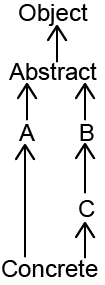
\includegraphics[width=.15\textwidth]{images/linear1.jpg}
		\caption{Inheritance hierarchy}
	}
	{
		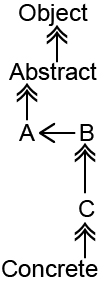
\includegraphics[width=.15\textwidth]{images/linear2.jpg}
		\caption{Linearization}
	}
\end{figure}
%end-twoCol



When we are invoking a method with a super chain (if any) the following, flattened chain, will be checked in order to satisfy an invocation: Concrete, C, B, A, Abstract, Object.

\textbf{Linearization algorithm}. It's not necessary to fully understand the details of the linearization algorithm in order to make use of stacked traits, but the algorithm itself is interesting...

Let's define the Linearization function, acting on a class $C$ as $Lin$:

\begin{center}
	$Lin(C) = C, Lin(C_n) \leftarrow \dots \leftarrow Lin(C_0)$
\end{center}

Where $C_0 \dots C_n$ denotes the superclass and composing traits of class $C$, defined on a left to right basis. The operator $\leftarrow$ is defined as follows:

\begin{center}
	\begin{align*}
		\left \{a, A \right \} \leftarrow B &= a, (A \leftarrow B) \text{ if } a \text{ is not inside } B\\
		&= A \leftarrow B \text{ if a is inside } B\text{, then } a \text{ is replaced by } B
	\end{align*}
\end{center}

Let's now look at this for class Concrete as defined above:

\begin{center}
	$Lin(Concrete) = Concrete, Lin(C) \leftarrow Lin(A) \leftarrow Lin(Abstract)$
\end{center}

Let's now recursivity apply the $Lin$ operator to each element on the right hand side of the above:

\begin{center}
	\begin{align*}
		Lin(Abstract) &= Abstract, Lin(Object)\\
		&= Abstract, Object\\
		\\
		Lin(A) &= A, Lin(Abstract)\\
		&= A, Abstract, Object\\
		\\
		Lin(C) &= C, Lin(B)\\
		&= C, B, Lin(Abstract)\\
		&= C, B, Abstract, Object
	\end{align*}
\end{center}

Putting this all together we arrive at the following:

\begin{center}
	$Lin(Concrete) = Concrete, C, B, Abstract, Object \leftarrow A, Abstract, Object \leftarrow Abstract, Object$
\end{center}

Finally, applying the $\leftarrow$ operator results in the following flattened, linearized, definition for Concrete:

\begin{center}
	$Lin(Concrete) = Concrete, C, B, A, Abstract, Object$
\end{center}

\section{Using non Concurnas traits/interfaces}
Traits may be defined and used within Concurnas to a limited extent. These may originate from other JVM languages such as Java, Kotlin etc. In the case of Java interfaces there are some caveats one needs to bear in mind when using them inside Concurnas:
\begin{itemize}
	\item They may not have non static state of any kind.
	\item They cannot be stacked.
	\item Superclass methods take precedence over trait methods if defined.
\end{itemize}

\end{document}